\chapter*{Ausarbeitung}

\section{Gezeitenpotential}

Gegeben sei der Punkt $P$ mit den sphärischen Koordinaten ($\lambda = 8.33^{\circ},~ \varphi = 48.14^{\circ},~r = 6366837~m$). Im Folgenden wird berechnet: 

\begin{enumerate}[a)]
\item Berechnung der Zeitreihe der Koeffizienten $v_{2,m}^{tid}$ 

Die Zeitreihe der Koeffizienten $v_{2,m}^{tid}$ vom Grad 2 des vom Mond erzeugten Gezeitenpotentials werden nun berechnet. Dabei werden explizit die Werte vom 15. Januar angegeben. Um die Zeitreihe zu berechnen wird folgende Formel herangezogen: 

\begin{gather*}
V^{tid}(\lambda, \phi, r) = \sum_{l=2}^{L} \sum_{m=-l}^{l} \left(\dfrac{r}{R}\right)^l v_{l,m}^{tid} \overline{Y}_{l,m}(\lambda,\phi) \\
v_{l,m}^{tid} = \dfrac{GM_{Moon}}{r_{Moon}} \dfrac{1}{2l+1} \left(\dfrac{R}{r_{Moon}}\right)^l \overline{Y}_{l,m} (\lambda_{Moon},\phi_{Moon}) \\
= \begin{bmatrix}
-0.5885 &  0.4409 &  -0.8039  & -0.0927 & -1.3381
\end{bmatrix}
\end{gather*} 

\item Berechnung des Gezeitenpotentials $v_{tid}$ 

Hier wird das vom Mond erzeugte Gezeitenpotential $v_{tid}$ berechnet. Anschließend werden die Zahlenwerte für den 1. bis 5. Januar angegeben. 

\begin{gather*}
v_{tid} = \begin{bmatrix}
-1.4564&-1.3540&-1.2456&-1.1379&-1.0388
\end{bmatrix}
\end{gather*}

\begin{figure}[H]
\centering
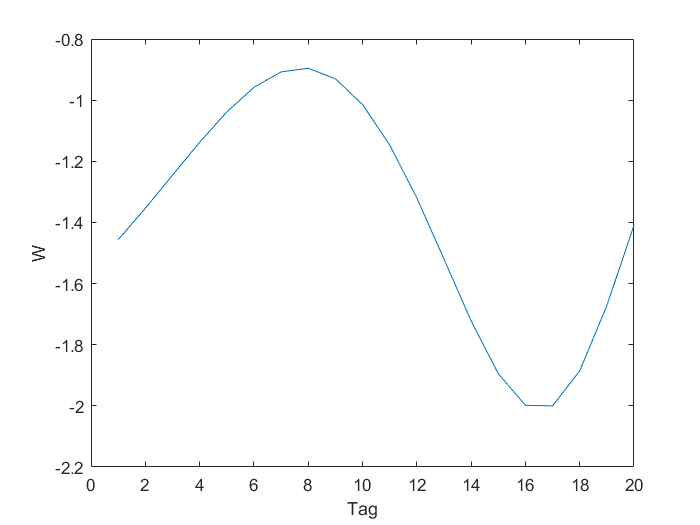
\includegraphics[scale=0.6]{gezpot.png}
\caption{Gezeitenpotential im Berechnungspunkt}
\label{gezpot}
\end{figure}

Abbildung \ref{gezpot} zeigt das Gezeitenpotential im Berechnungspunkt für das gesamte Zeitintervall im Januar. 

\item Berechnung des Gezeitenvektors $g_{tid}$

Nun wird der zugehörige Gezeitenvektor $g_{tid}$ für den 20. Januar berechnet. Dabei wird das ganze auf Terme vom Grad 2 beschränkt. 

\begin{gather*}
g_{tid} = \begin{bmatrix}
-0.4434 &-0.1148 &-0.9148
\end{bmatrix}
\end{gather*}
\end{enumerate}

\section{Gezeitenkatalog HW95}

Aus dem Gezeitenkatalog HW95, welches 12935 Partialtiden der Sonne, des Mondes und einiger Planeten enthält, soll das vom Mond erzeugte Gezeitenpotential $v_{tid}$, sowie der zugehörige Gezeitenvektor $g_{tid}$ für denselben Beobachtunspunkt und dieselben Zeitpunkte wie in Aufgabe 1 berechnet werden. 

